\section{Prognosis: does the map predict?}
\label{sec:prognosis}

The previous chapter showed the map and its strata \emph{persist}; this one asks whether they
\emph{predict}. The distinction is the whole point of the program: a description can be stable and still
clinically idle. The question is sharp and deliberately conservative --- does a baseline coordinate or
stratum forecast a future clinical outcome \emph{incrementally beyond what a clinician already has}, namely
the DSM-5 diagnosis, the current severity, and the present value of the outcome itself? The bet, placed
exactly where temporal coherence pointed, is that the \emph{durable} trait axes (cognition, metabolic,
inflammatory) predict the \emph{moving} state outcomes (functioning, severity). Throughout, this chapter is
a pure consumer of the fixed objects from the earlier chapters --- the panel of re-scored coordinates,
their per-patient uncertainty, the archetype memberships, and the attrition weights --- never re-estimated
(invariant I3). The outcomes are clinical scales re-administered over the dense yearly grid
V0\,$\to$\,V2; there is no hospitalization or relapse register in the record, so the forecasts are of
\emph{scale trajectories}, not events (\S\ref{sub:m4limits}).

\subsection{The estimand and the bar}
For an outcome $Y$ at the two-year horizon we fit a strictly nested ladder, every rung on one
complete-case sample so the held-out fit is comparable: nuisance (age, sex, a site random intercept)
$\to$ {}$+$\,DSM-5 subtype $\to$ {}$+$\,severity $\to$ {}$+$\,the baseline outcome $Y_0$. That last
rung --- call it the \emph{bar} --- is an analysis of covariance: by conditioning on $Y_0$ it asks what
predicts the future \emph{given where the patient is now}, which both answers the clinically honest
question and disarms regression to the mean. The transdiagnostic map is then added on top, as continuous
durable coordinates or as archetype/tessellation memberships, and credited only if it beats the bar.

\begin{methodsbox}[Errors-in-variables: the map's uncertainty is propagated, not ignored]
A coordinate is a posterior, not a point. Plugging its mean into a regression would attenuate the
coefficient toward zero --- the textbook \emph{regression-dilution} effect, in which noise in a predictor
flattens its apparent slope, and the damage is worst exactly where the coordinate is least certain. The
remedy is to trust each reading in proportion to its precision: each map predictor enters as a latent true
value carrying the \emph{known} per-patient standard deviation from the map (the variance-model device of
Eq.~\ref{eq:traitstate}, generalized to the outcome equation):
\begin{equation}
\label{eq:eiv}
g\!\left(\mathbb{E}[Y_{i}]\right)=\alpha+\mathbf{x}_i^{\!\top}\bm\beta+u_{\mathrm{site}(i)}+\xi_i\,\beta_{z},
\qquad z_{i}\sim\Normal\!\left(\xi_i,\,s^2_{i}\right),\quad \xi_i\sim\Normal(\mu,\tau^2),
\end{equation}
so a wide-posterior coordinate self-down-weights and $\beta_z$ is attenuation-corrected. Severity enters
the same way through the \emph{error-corrected} general factor $G$ --- the move that lets Q2 answer ``is
it just baseline severity, measured noisily?''. Discrimination is then re-expressed in the clinician's
currency by patient-level cross-validated logistic models (AUC, calibration, net benefit).
\end{methodsbox}

\subsection{The map adds for functioning, not severity (Q1)}
On the bar (DSM-5 $+$ severity $+$ baseline outcome), added value splits cleanly by outcome.

\begin{keyresult}[The transdiagnostic profile predicts two-year functioning]
For \textbf{functioning} (EGF, $N=2{,}114$) the eight archetypes add held-out $\Delta$ELPD $\mathbf{+46}$
--- expected log predictive density, a measure of out-of-sample predictive accuracy (higher is better), so
$+46$ log-likelihood units of held-out fit beyond the bar --- in the $G$-residualized Arm-B view ($+58$ for
the full-phenotype Arm-A), with the four-region tessellation $+47$ --- clearly predictive. The durable \emph{biology} coordinates carry it: metabolic
$\beta=-0.062\,[-0.103,-0.022]$ and inflammatory $-0.060\,[-0.112,-0.011]$ both exclude zero (higher
load $\to$ worse future functioning). For \textbf{severity} (CGI-S, $N=2{,}345$) the map adds essentially
nothing: severity is autoregression-saturated --- today's CGI-S and $G$ already fix it.
\end{keyresult}

The strata out-predict the three linear coordinates because they capture the \emph{multivariate corner}
a patient occupies, which three additive terms cannot. That the continuous durable trio is individually
credible (above) yet adds little \emph{held-out ELPD} ($+7$, ambiguous) is the first sign of a theme
(\S\ref{sub:m4value}): the map's value is multivariate and group-level, not a large per-axis effect.

\subsection{Beyond severity --- the biology is the clean signal (Q2)}
The load-bearing test is whether the biology effect is more than baseline severity in disguise. It is:
metabolic survives adjustment for the \emph{error-corrected} $G$ severity ($\beta=-0.055\,[-0.095,-0.015]$)
as well as the manifest CGI-S. This is the central bet of the map --- biology largely independent of $G$ --- cashed
out prognostically: the metabolic/inflammatory corner a patient \emph{keeps} (the trait, from the temporal
chapter) forecasts the functional state they \emph{move toward} (the state). Cognition does not reach
credibility (prior-dominated for the untested, and the weakest of the three).

\subsection{Versus DSM-5: complementary, and course-dependent (Q3)}
The deferred G5 test, now answerable because outcomes (unlike the enrolment diagnosis) move. On a shared
foundation we fit four nested models --- foundation, $+$DSM-5, $+$map, $+$both --- and read the
\emph{dominance asymmetry} (Figure~\ref{fig:m4dominance}).

\begin{figure}[h]\centering
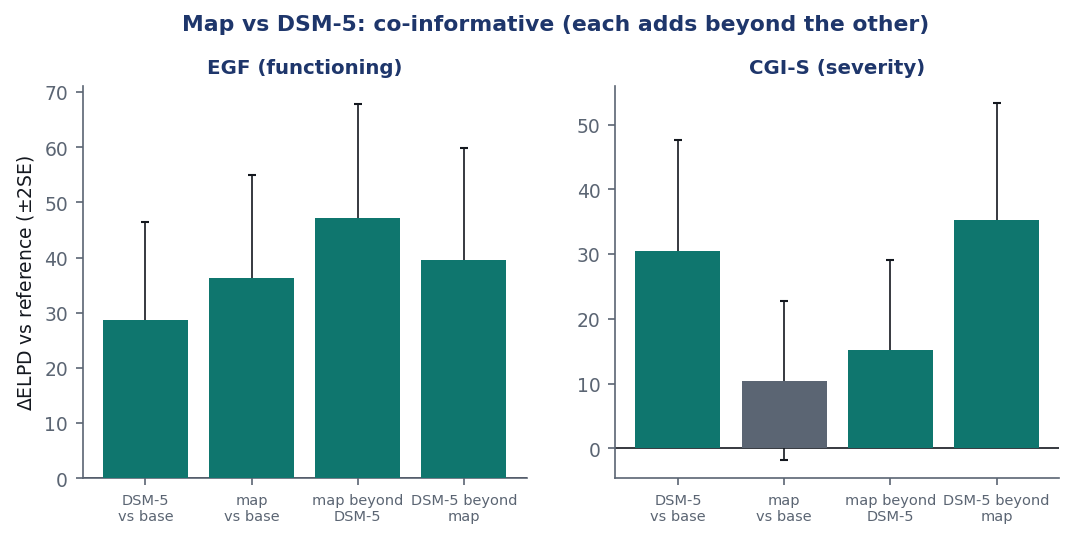
\includegraphics[width=0.92\linewidth]{figures/m4_dominance.png}
\caption{Map versus the seven DSM-5 subtypes, on top of nuisance $+$ severity $+$ baseline outcome. For
functioning the map adds beyond DSM-5 (\emph{map beyond DSM-5}, $+47$) \emph{and} DSM-5 adds beyond the
map (\emph{DSM-5 beyond map}, $+40$): they are \textbf{co-informative}, not rivals. For severity both
shrink and DSM-5 leads. Bars clearing $2\,$SE in teal.}
\label{fig:m4dominance}
\end{figure}

\begin{keyresult}[Co-informative with DSM-5, and concentrated where the future is open]
The map and the DSM-5 subtypes each carry prognostic information the other lacks --- diagnosis the
categorical illness type, the largely $G$-independent map the dimensional biology profile --- so the map
\emph{complements}, it does not replace, diagnosis (consistent with the program's four-layer design, in
which diagnosis stays metadata). And the added value is \textbf{course-dependent}: large within bipolar
($\Delta$ELPD $+43$) and depression, null within schizophrenia ($-1.8$). The schizophrenia null is
\emph{foundation saturation}, not map failure --- its baseline already explains more ($R^2\,0.26$ vs
bipolar's $0.17$), with matched outcome variance and coordinate spread. The map predicts where the
trajectory is not already fixed by baseline severity.
\end{keyresult}

\subsection{The prognostic atlas --- the clinical ``so what''}
\label{sub:m4atlas}
The value a clinician reads is not a $\Delta$ELPD but a difference in outcome between groups. Assigning
each patient to their dominant archetype yields a prognostic atlas (Figure~\ref{fig:m4atlas}):
two-year functional remission ranges from \textbf{14\%} (the suicidality archetype) to \textbf{60\%} (the
low-burden archetype) --- a four-fold spread that a single autoregressive coefficient hides --- and
\emph{every} archetype is transdiagnostic, drawing patients from all three cohorts. On the separation of
outcomes the division of labour is intuitive: the archetypes separate the \emph{dynamic transitions}
(remission, deterioration, relapse) better than the DSM-5 subtypes, while the subtypes separate the
\emph{severity-level} outcomes (who stays chronically ill) better --- the same co-informative split, in
the clinic's own units.

\begin{figure}[h]\centering
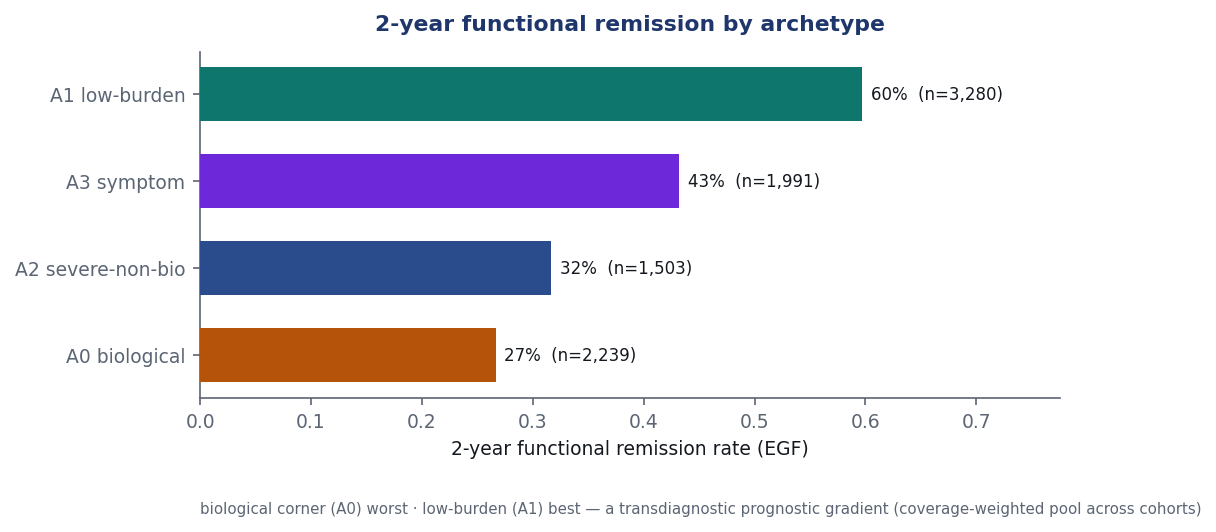
\includegraphics[width=0.96\linewidth]{figures/m4_atlas.png}
\caption{The archetype prognostic atlas: per-archetype rate of each two-year clinical endpoint
(remission/recovery good $\uparrow$; deterioration/sustained/relapse adverse $\downarrow$), coloured by
adversity (blue favourable, red adverse). Archetypes ordered by functional-remission rate; the
low-burden corner remits and the suicidality/inflammatory corners persist. The trajectories diverge over
follow-up while keeping rank --- the trait/state geometry from the temporal chapter, now in outcomes.}
\label{fig:m4atlas}
\end{figure}

\subsection{Is it worth using? Discrimination, calibration, net benefit}
\label{sub:m4value}
The honest counterweight to the atlas. Cross-validated, the clinician's reference already predicts these
endpoints well (AUC $0.73$--$0.87$); adding the map gives a \emph{small but reliable} discrimination gain
only for functional remission, and nothing where the reference is already strong
(Figure~\ref{fig:m4value}, Table~\ref{tab:m4value}).

\begin{figure}[h]\centering
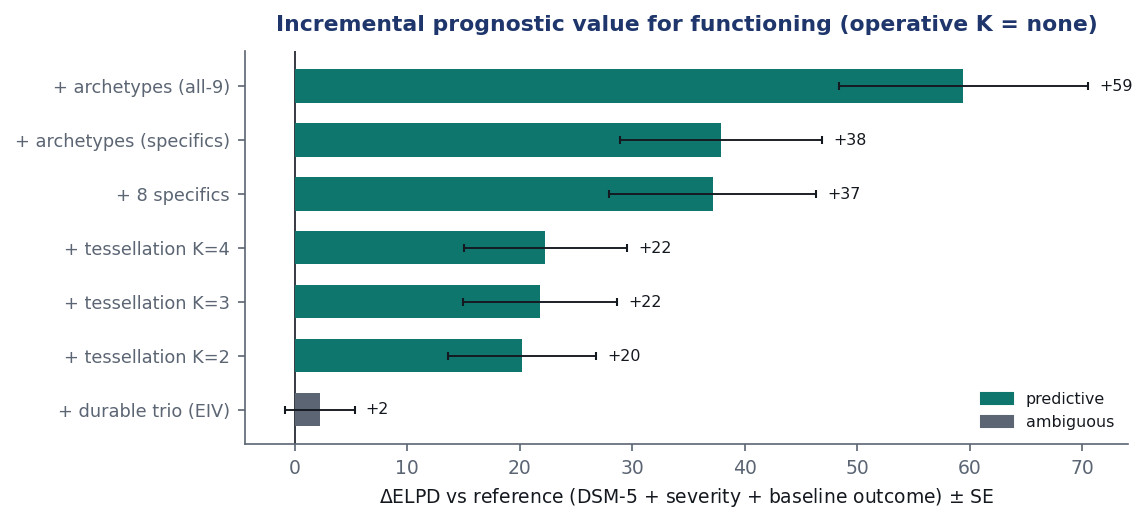
\includegraphics[width=0.9\linewidth]{figures/m4_value.png}
\caption{Discrimination (5-fold cross-validated AUC) of the four endpoints. Neither DSM-5 alone nor the
map alone is a strong classifier; the reference (diagnosis $+$ severity $+$ baseline) carries most of it,
and \emph{reference $+$ map} edges it for functional remission.}
\label{fig:m4value}
\end{figure}

\begin{table}[h]\centering\small\sffamily
\caption{Clinical value of adding the map to the reference. AUC is patient-level 5-fold cross-validated;
$\Delta$AUC is the paired gain with a bootstrap interval. The map's reliable individual increment is
functional remission; the large signal is the group-level atlas (\S\ref{sub:m4atlas}), not binary
discrimination. The gap between ``$+46$ $\Delta$ELPD'' and ``$+0.017$ $\Delta$AUC'' is the cost of
collapsing the functional continuum to one threshold.}
\label{tab:m4value}
\begin{tabular}{L{4.0cm} R{1.6cm} R{1.6cm} R{2.6cm} L{2.0cm}}
\toprule
\hdr{endpoint} & \hdr{ref. AUC} & \hdr{$+$map AUC} & \hdr{$\Delta$AUC (map)} & \hdr{verdict}\\
\midrule
\rowcolor{facebg} functional remission & 0.76 & 0.78 & $+0.017\,[.009,.026]$ & reliable\\
sustained impairment & 0.83 & 0.84 & $+0.008\,[.000,.015]$ & marginal\\
\rowcolor{facebg} deterioration & 0.73 & 0.73 & $+0.003$ & none\\
relapse surrogate & 0.87 & 0.87 & $+0.002$ & none\\
\bottomrule
\end{tabular}
\end{table}

\subsection{Robustness: does the headline survive? (Q4)}
The functioning result survives the obvious threats (Table~\ref{tab:m4robust}). Under inverse-probability
weighting for attrition the durable coefficients are essentially unchanged (metabolic $-0.062\to-0.059$),
they hold when restricted to well-measured patients (so it is not a prior-dominated-coordinate artefact),
and the durable block's incremental fit exceeds a permutation null ($p=0.001$). The one boundary is
honest and already named: dropping bipolar --- the cohort that carries the open-course signal --- widens
the intervals across zero, the course-dependence of Q3 confirmed rather than hidden.

\begin{table}[h]\centering\small\sffamily
\caption{Robustness of the durable biology effect on functioning (EIV $\beta$, 94\% interval) and of the
functional-remission AUC gain. Survives attrition, reliability restriction, and a permutation null;
weakens dropping bipolar (course-dependence). $^{\ast}$interval excludes zero.}
\label{tab:m4robust}
\begin{tabular}{L{4.6cm} R{2.6cm} R{2.6cm} R{2.2cm}}
\toprule
\hdr{check} & \hdr{metabolic $\beta$} & \hdr{inflammatory $\beta$} & \hdr{$\Delta$AUC}\\
\midrule
\rowcolor{facebg} baseline & $-0.062^{\ast}$ & $-0.060^{\ast}$ & $+0.017$\\
IPW (attrition) & $-0.059^{\ast}$ & $-0.056^{\ast}$ & $+0.016$\\
\rowcolor{facebg} reliability (well-measured) & $-0.059^{\ast}$ & $-0.060^{\ast}$ & ---\\
permutation null & \multicolumn{2}{c}{real $\Delta R^2\,0.006$ vs null $0.003$, $p=0.001$} & ---\\
\rowcolor{facebg} leave-out bipolar & $-0.047$ & $-0.065$ & $-0.001$\\
\bottomrule
\end{tabular}
\end{table}

\subsection{What prognosis establishes --- and what it defers}
\label{sub:m4limits}
On the fixed map, a baseline transdiagnostic profile predicts two-year \emph{functional} trajectory
incrementally beyond diagnosis and severity --- robustly, complementarily to DSM-5, and concentrated in
the patients whose course is not already fixed by baseline severity (Table~\ref{tab:m4goals}). Severity
itself is baseline-determined, and the map's worth is a \emph{stratification} (the atlas) plus continuous
forecasting, not a large individual-binary boost.

\begin{table}[h]\centering\small\sffamily
\caption{The prognosis gates and verdicts (internal validity, V0$\to$V2; functioning as the primary outcome).}
\label{tab:m4goals}
\begin{tabular}{L{2.1cm} L{5.3cm} L{5.4cm}}
\toprule
\hdr{gate} & \hdr{question} & \hdr{verdict}\\
\midrule
\rowcolor{facebg} Q1 incremental & adds beyond diagnosis $+$ severity? & yes for functioning ($+46$ ELPD); no for severity\\
Q2 beyond severity & survives error-corrected severity? & yes --- metabolic $\beta$ holds under $G$\\
\rowcolor{facebg} Q3 vs DSM-5 & better than / across the subtypes? & co-informative; course-dependent (BP/DR, not SZ)\\
Q4 robust & survives attrition / reliability / chance? & yes; weakens dropping bipolar (honest)\\
\bottomrule
\end{tabular}
\end{table}

\begin{openbox}[Prediction is not moderation --- that comes next]
This chapter shows the map \emph{forecasts} who will do well; it does not show it \emph{changes what to do}.
Whether a stratum \emph{moderates treatment response} --- the stratum-by-treatment interaction, the point
at which a phenotype alters management --- is the final chapter's question, and it will require a treatment
or randomization variable the present record may not contain (the enrolment \texttt{arm} is a DSM-5 subtype,
not an assigned treatment). Caveats carried forward: scale trajectories, not events; internal association, not a
validated or causal decision rule; bipolar/depression-concentrated, with the rare archetypes
(inflammatory, suicidality) wide; a two-year horizon. \emph{Predicts $\ne$ moderates.}
\end{openbox}
